\section{Visitor-Muster}
Verwenden Sie das Visiotr-Muster, wenn Sie ein Objekt-Kompositum um neue F"ahigkeiten erweitern m"ochten und neue Kapselung unwichtig ist.

\subsection{Problemstellung}
Die G"aste, die das Restaurant und das Pfannkuchenhaus besuchen, sind in letzter Zeit gesundheitsbewusster geworden. Bevor sie ihr Essen bestellen, fragen sie nach Nahrungsmittelinformationen. Da beide Restaurantsbereit sind Sonderbestellungen entgegenzunehmen, fragen manche G"aste sogar nach Nahrungsmittelinformationen zu einzelnen Zutaten.

\subsection{Erkl"arung des Musters}
Der Visitor muss jedes Element des Kompositums besuchen; diese Funktionalit"at steckt in einem Durchquerer-Objekt. Der Visitor wird von Durchquerer angeleitet, den Zustand von allen Objekten im Kompositum zu erfassen. Wenn der Zustand einmal erfasst ist, kann der Client den Visitor verschiedene Operationen auf dem Zustand ausf"uhren lassen. Ist neue Funktional"at erforderlich, muss lediglich der Visitor erweiter werden.

\begin{figure}
	\centering
	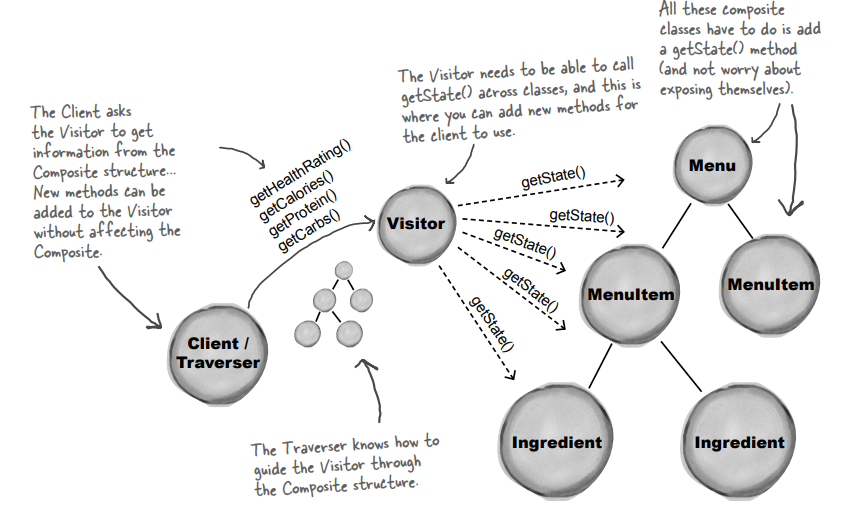
\includegraphics[width=\linewidth]{visitor/img/visitorUML}
	\caption{UML-Darstellung des Visitor-Musters}
	\label{fig:visitorUML}
\end{figure}

\subsection{Vorteile}
\begin{enumerate}
\item Erm"oglicht Operationen zu einer Kompositumsstruktur hunzuzuf"ugen, ohne die Struktur selbst zu "andern.
\item Das Hinzuf"ugen neuer Operationen ist relativ einfach
\item Der Code f"ur Operationen, die der Visitor durchf"uhrt, ist zentralisiert.
\end{enumerate}

\subsection{Nachteile}
\begin{enumerate}
\item Bei der Verwendung des Visitors wird die Kapselung der Kompositumsklassen zerst"ort.
\item Da die Durchquererfunktion mit in die Sache verwickelt ist, sind die Ver"anderungen an der Kompositumsstruktur schwieriger.
\end{enumerate}

